%!TEX root = paper.tex

\section{Results}\label{sec:results}

In this section we present and discuss our five submitted images. The images have been generated from the source images which are shown in Figure \ref{fig:source_images}.

Alongside each submitted image we appended a .conf file which contains the exact command line call which was used to generate the respective image. The submitted images are shown in Figure \ref{fig:submitted}. For comparison an image of the target classes is displayed beneath each of them.

\begin{figure}
\centering
\begin{subfigure}{.19\linewidth}
  \centering
  
\includegraphics[width=0.7\linewidth]{imgs/octocat}
\end{subfigure}
\begin{subfigure}{.19\linewidth}
  \centering
  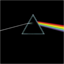
\includegraphics[width=0.7\linewidth]{imgs/darkside}
\end{subfigure}
\begin{subfigure}{.19\linewidth}
  \centering
  
\includegraphics[width=0.7\linewidth]{imgs/gi}
\end{subfigure}
\begin{subfigure}{.19\linewidth}
  \centering
  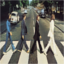
\includegraphics[width=0.7\linewidth]{imgs/abbey}
\end{subfigure}
\begin{subfigure}{.19\linewidth}
  \centering
  
\includegraphics[width=0.7\linewidth]{imgs/die_???}
\end{subfigure}
\caption{Source images}
\label{fig:source_images}
\end{figure}

\begin{figure}[!h]
\centering
\begin{subfigure}{.19\linewidth}
  \centering
  
\includegraphics[width=0.7\linewidth]{imgs/4}
\end{subfigure}%
\begin{subfigure}{.19\linewidth}
  \centering
  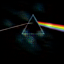
\includegraphics[width=0.7\linewidth]{imgs/7}
\end{subfigure}
\begin{subfigure}{.19\linewidth}
  \centering
  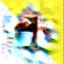
\includegraphics[width=0.7\linewidth]{imgs/10}
\end{subfigure}
\begin{subfigure}{.19\linewidth}
  \centering
  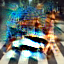
\includegraphics[width=0.7\linewidth]{imgs/16}
\end{subfigure}
\begin{subfigure}{.19\linewidth}
  \centering
  
\includegraphics[width=0.7\linewidth]{imgs/20}
\end{subfigure}

\begin{subfigure}{.19\linewidth}
  \centering
  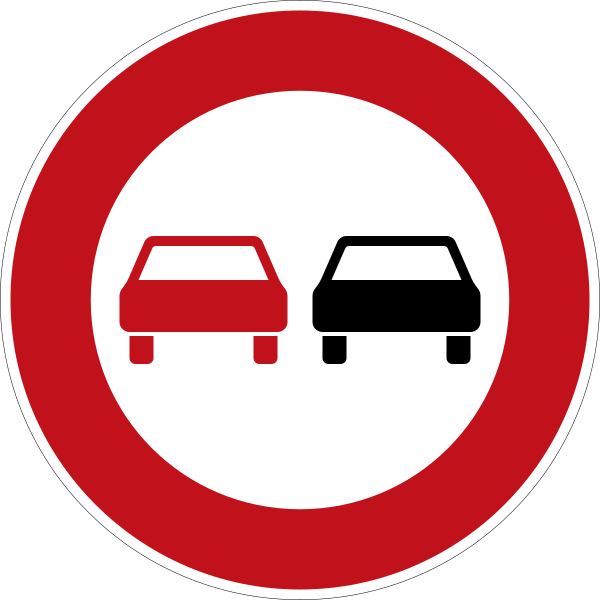
\includegraphics[width=0.7\linewidth]{imgs/4_real}
\end{subfigure}%
\begin{subfigure}{.19\linewidth}
  \centering
  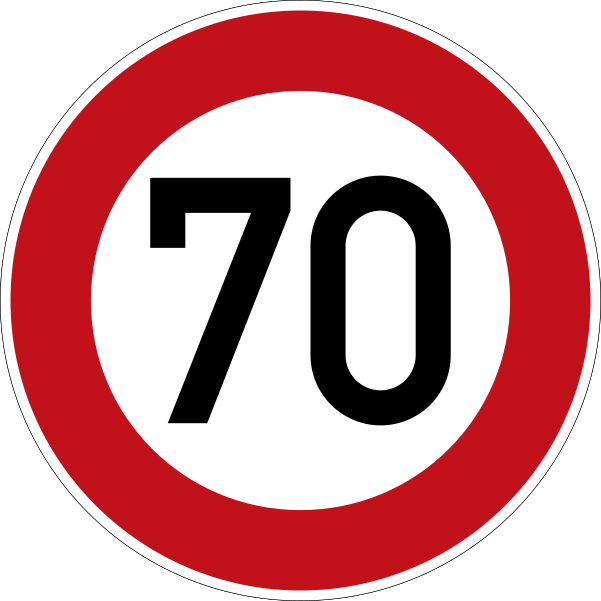
\includegraphics[width=0.7\linewidth]{imgs/7_real}
\end{subfigure}
\begin{subfigure}{.19\linewidth}
  \centering
  
\includegraphics[width=0.7\linewidth]{imgs/10_real}
\end{subfigure}
\begin{subfigure}{.19\linewidth}
  \centering
  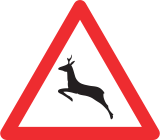
\includegraphics[width=0.7\linewidth]{imgs/16_real}
\end{subfigure}
\begin{subfigure}{.19\linewidth}
  \centering
  
\includegraphics[width=0.7\linewidth]{imgs/20_real}
\end{subfigure}
\caption{Submitted images}
\label{fig:submitted}
\end{figure}

\begin{enumerate}
\item
\textbf{Überholverbot für Kraftfahrzeuge aller Art: 99.99 \%}

The first adversarial example was generated from Git\-Hub's octocat using the Carlini \& Wagner L2 algorithm on a substitute model,
which was trained on the GTSRB training data.
It does not resemble the target sign at all and the source image is clearly recognizable.

\item
\textbf{Zulässige Höchstgeschwindigkeit (70): 99.41\%}

The second example was generated from the album cover of Pink Floyd's "The Dark Side of the Moon".
It uses the same setup as the first image.
Although there exists some noise on the black background, the target image is not recognizable and the album cover is still clearly visible.

\item
\textbf{Gefahrenstelle: $\approx$100\%}

\begin{figure}[!h]
\centering
\begin{subfigure}{.19\linewidth}
  \centering
  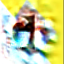
\includegraphics[width=0.7\linewidth]{imgs/robust_10/0_ll}
  \caption{99.97\%}
\end{subfigure}
\begin{subfigure}{.19\linewidth}
  \centering
  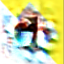
\includegraphics[width=0.7\linewidth]{imgs/robust_10/1_l}
  \caption{$\approx$100\%}
\end{subfigure}
\begin{subfigure}{.19\linewidth}
  \centering
  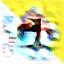
\includegraphics[width=0.7\linewidth]{imgs/robust_10/2_c}
  \caption{95.03\%}
\end{subfigure}
\begin{subfigure}{.19\linewidth}
  \centering
  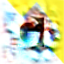
\includegraphics[width=0.7\linewidth]{imgs/robust_10/3_r}
  \caption{99.85\%}
\end{subfigure}
\begin{subfigure}{.19\linewidth}
  \centering
  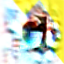
\includegraphics[width=0.7\linewidth]{imgs/robust_10/4_rr}
  \caption{99.98\%}
\end{subfigure}
\end{figure}

The third adversarial example is based on the GI logo.
It was constructed using the modified Carlini \& Wagner attack,
which modifies an image from multiple perspectives simultaneously.
The attack was performed on the model, which was trained using Jacobian based dataset augmentation.

The generated images are heavily perturbed;
yet, the GI logo is still noticeable while the target class is not recognizable.

\item
\textbf{Wildwechsel: 100\%}

\begin{figure}[!h]
\centering
\begin{subfigure}{.19\linewidth}
  \centering
  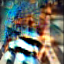
\includegraphics[width=0.7\linewidth]{imgs/robust_16/0_ll}
  \caption{97.62\%}
\end{subfigure}
\begin{subfigure}{.19\linewidth}
  \centering
  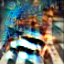
\includegraphics[width=0.7\linewidth]{imgs/robust_16/1_l}
  \caption{100\%}
\end{subfigure}
\begin{subfigure}{.19\linewidth}
  \centering
  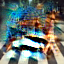
\includegraphics[width=0.7\linewidth]{imgs/robust_16/2_c}
  \caption{100\%}
\end{subfigure}
\begin{subfigure}{.19\linewidth}
  \centering
  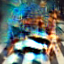
\includegraphics[width=0.7\linewidth]{imgs/robust_16/3_r}
  \caption{100\%}
\end{subfigure}
\begin{subfigure}{.19\linewidth}
  \centering
  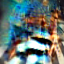
\includegraphics[width=0.7\linewidth]{imgs/robust_16/4_rr}
  \caption{99.99\%}
\end{subfigure}
\end{figure}

The fourth adversarial example uses the same attack as the third, but is performed on the GTSRB-model.
It was generated from the Beatle's "Abbey Road" album cover.

Though the zebra crossing is still visible on closer inspection, the original image is too heavily perturbed to be identifiable. 
Nevertheless, the adversarial example does not resemble the target class (nor any other traffic sign) and is therefore valid.

\item
\textbf{Vorfahrt: 99.99\%}

\begin{figure}[!h]
\begin{subfigure}{.19\linewidth}
  \centering
  
\includegraphics[width=0.7\linewidth]{imgs/die_???}
  \caption{Source}
\end{subfigure}
\hspace{0.05\linewidth}
\begin{subfigure}{.19\linewidth}
  \centering
  
\includegraphics[width=0.7\linewidth]{imgs/inv_???mask}
  \caption{Mask}
\end{subfigure}
\hspace{0.05\linewidth}
\begin{subfigure}{.19\linewidth}
  \centering
  
\includegraphics[width=0.7\linewidth]{imgs/20}
  \caption{Result}
\end{subfigure}
\end{figure}

The last image was created by the robust physical attack (RP$_2$) applied to the GTSRB-model.
It was generated from the logo of the three investigators (Die Drei Fragezeichen) where the question marks have been masked (i.e. they remain unperturbed).
The final image is not recognizable as a traffic sign.

\end{enumerate}
